\documentclass[degree=doctor,bibtype=numeric]{tongjithesis}
% 选项:
%   degree=[master|doctor], 							% 必选
%   bibtype=[numeric|authoryear], 						% 可选,数字式引用|作者-年份引用,默认为数字式(上标)引用
%   degreetype=[academic|profession|equaleducation],  	% 可选, 学术型|专业型|同等学力,默认为学术型
% 	electronic,                                 		% 可选, 电子版,(打印时删除)
%   secret,                                     		% 可选,是否保密,基本不用
%   pifootnote,                                 		% 可选,默认已打开
%   romantitle                                  		% 可选,默认已打开
%   注:默认已打开的选项可以使用arialtitle=false的形式关闭。

% 所有其它可能用到的包都统一放到这里了,可以根据自己的实际添加或者删除。
\usepackage{tongjiutils}

%参考文献更新使用biblatex包, 使用gb7714-2015标准, 具体参数设置可在cls文件中搜索biblatex进行了解
%加入bib文件(老版本文件依然能够使用)
\addbibresource{ref/refs.bib}   %


\begin{document}

% 定义所有的eps文件在 figures 子目录下
\graphicspath{{figures/}}


%%% 封面部分
\frontmatter
\tongjisetup{
  %******************************
  % 注意:
  %   1. 配置里面不要出现空行
  %   2. 不需要的配置信息可以删除
  %******************************
  %
  %=====
  % 密级
  %=====
  secretlevel={保密},
  secretyear={2},
  %
  %=========
  % 中文信息
  %=========
  % 题目过长可以换行(推荐手动加入换行符,这样就可以控制换行的地方啦)。
  ctitle={基于结构与状态的电网脆弱性\\综合评估模型研究},
  cheadingtitle={基于结构与状态的电网脆弱性综合评估模型研究},    %用于页眉的标题,不要换行
  cauthor={李炅聪},
  studentnumber={1732929},
  cmajorfirst={工程},
  cmajorsecond={控制工程},
  cdepartment={电子与信息工程学院},
  csupervisor={苏永清~~~副教授},
  % 如果没有副指导老师或者校外指导老师,把{}中内容留空即可,或者直接注释掉。
  %cassosupervisor={裴刚 教授~(校外)}, % 副指导老师
  % 日期自动使用当前时间,若需手动指定,按如下方式修改:
  % cdate={\zhdigits{2018}年\zhnumber{11}月},
  % 没有基金的话就注释掉吧。
  %cfunds={(本论文由我要努力想办法撑到两行的著名国家杰出青年基金 (No.123456789) 支持)},
  %
  %=========
  % 英文信息
  %=========
  %etitle={Research on Vulnerability Analysis and \\Quantitative Evaluation of Power System \\Based on Complex Network},
  etitle={Research on Comprehensive Assessment Model \\of Power Grid Vulnerability \\Based on Structure and State},
  eauthor={Li Jiongcong},
  emajorfirst={Engineering},
  emajorsecond={Control Engineering},
  edepartment={College of Electronics and ~~~~~~~~~~~~~~~~Information Engineering},
%emajorfirst{Control Science and Engineering}
%emajorsecond{Control Theory and Control Engineering}
  % 日期自动使用当前时间,若需手动指定,按如下方式修改:
  % edate={November,\ 2018},
  %efunds={(Supported by the Natural Science Foundation of China for\\ Distinguished Young Scholars, Grant No.123456789)},
  esupervisor={A. Prof.  Su Yongqing},
  %eassosupervisor={Prof. Gang Pei (XiaoWai)}
  }

% 定义中英文摘要和关键字
\begin{cabstract}
电力系统作为维持国计民生的重要组成部分,其稳定性、可靠性及安全性至关重要。近年来,世界各地发生的多起大停电事故也引起越来越多专家学者的关注。研究表明,大多数大停电事故的发生原因是局部故障。
% 结构和状态是电网脆弱性研究的两个重要方面,电网结构的完整性是维持电网稳定运行的基础,电网状态的不稳定会导致局部故障的发生。
因此,综合评估和识别电网的脆弱环节并采取有效控制措施是避免大停电事故发生的关键。在此背景下,本文针对基于结构与状态的电网脆弱性综合评估模型展开研究,主要工作归纳如下:

% 在电力系统运行过程中,脆弱性是其固有属性,在扰动因素作用下,电网自身固有的脆弱性显现的概率大增,将对其稳定运行
% 造成威胁,因此有必要分析电力系统的脆弱性,识别电力系统的脆弱环节,科学合理地评估电网脆弱环节的脆弱性程度,对其进行结构优化和重点防护,保证电网稳定可靠运行。

本文研究了复杂网络特征参数和网络模型,验证分析电力系统的小世界性和无标度性。通过阐述复杂网络脆弱性概念得出,复杂网络的脆弱性在于其子系统的存在性,明确了本文研究的关键问题。

通过查阅各领域脆弱性相关文献,结合复杂网络脆弱性概念和电力系统脆弱性特征,得出较为清晰的电力系统脆弱性定义,并进行脆弱过程分析及数学描述。从结构和状态两个方面对系统脆弱性进行研究,
在结构方面,基于复杂网络理论建立电力系统拓扑模型,并提出结构脆弱性指标,建立了电网结构脆弱性模型;在状态方面,从节点电压稳定性、过负荷能力和电网损耗方面提出状态脆弱性指标,并建立电力
系统负荷模型,通过蒙特卡洛方法对状态脆弱性指标进行计算分析,建立了电网状态脆弱性模型。

建立电力系统脆弱性评估指标体系,分别选取反映系统脆弱性的结构和状态脆弱性指标进行分析,并对其归一化处理,采用改进熵权法和离差最大化法分别对结构脆弱性指标集和状态脆弱性指标集
进行权重分配和指标融合得到了脆弱性一级指标,进一步利用D-S证据理论对一级指标进行融合,建立了基于结构与状态的电网脆弱性综合评估模型。

最后,以$IEEE39$系统为研究对象,依据本文建立的电网脆弱性综合评估模型,
结合算例系统结构和参数分别对电力系统的结构和状态脆弱性进行分析,得到了结构脆弱性和状态脆弱性分析结果。最后,基于聚类算法和系统脆弱性综合评估结果进行脆弱节点等级评估,
根据得到的系统综合脆弱性等级评估结果,识别系统的脆弱环节。
% 针对电网结构脆弱性,本文制定了电网蓄意攻击策略,以$IEEE118$系统为研究对象,通过 MATLAB 算例仿真实验得出最优蓄意攻击策略,验证了结构脆弱性指标的合理性及重要性。
\end{cabstract}

\ckeywords{复杂网络,结构脆弱性,状态脆弱性,综合评估模型,脆弱环节识别}

\begin{eabstract}

\end{eabstract}

\ekeywords{} 
\makecover


% 目录
\tableofcontents
% 符号对照表
\begin{denotation}
\item[GNU] GNU's Not Unix /'gnu:/
\item[GFDL] GNU Free Documentation License
\item[GPL] GNU General Public License
\item[FSF] Free Software Foundation
\item[SMP] 对称多处理
\item[API] 应用程序编程接口
\item[$E$] 能量
\item[$m$] 质量
\item[$c$] 光速
\item[$P$] 概率
\item[$T$] 时间
\item[$v$] 速度

\end{denotation}

%%% 以下索引按需要选择
% 插图索引
\listoffigures
% 表格索引
\listoftables
% 公式索引
% \listofequations

%%% 正文 
\mainmatter
\chapter{绪论}

\section{研究背景与研究意义}
\label{sec:research_background}
随着社会的发展,人民生活和现代化水平的不断提高,导致对电能的需求越来越大,电力系统作为维持国计民生的重要组成部分,其稳定运行、经济性、可靠性以及安全性越来越重要。
近年来,随着电力系统规模的不断扩大和电力系统复杂性的逐步增加,使得电力系统各元件之间的关联越来越紧密。电力系统在促进社会发展和人民生活水平提高的同时,由于某一局
部故障而导致电网的连锁性崩溃,甚至导致大停电事故的例子屡见不鲜,从这方面来讲,这些电网故障不仅带来巨大的经济损失,还将严重影响社会经济的发展和人民的生活水平的提高。

自进入21世纪后,全球各地发生了很多大面积电网瘫痪事故。在国内,近年来,对社会经济和人民生活影响最大电网故障要数2008年南方特大雪灾导致的全国大范围停电事故了,这一年
我国遭遇了50年一遇的冰雪灾害,由于暴雪、冻雨导致华南地区、华中和华北部分地区输变电线路出现大范围断线倒塔,造成大范围停电限电,严重影响了电网安全运行,有地区甚至断
水断电十余天,引发交通运输、物资调度、等方面的连锁反应,严重影响了人们的日常生活,影响人数达2亿人。据调查统计,此次灾害导致停运电力线路37606条,停运的变电站共2027
座,111--500~kV线路倒塌8165座,给南方地区造成了巨大的经济损失。
在国外,2018年3月21日,巴西电网发生大面积停电事故,涉及巴西北部与东北部14个州,其中受影响最为严重的是贝里奥格兰德州、帕拉伊巴州和马拉尼昂州。在此次停点事故中,北部
和东北部电网与主网裂解,最终损失负荷21735~MW,相当于巴西互联电网停电前负荷的27\%,全国约四分之一的用户断电。事故原因为巴西欣古换流站交流测500~kV断路器故障\cite{refs1}。
此外,近期发生的“3.7”委内瑞拉停电事故,委内瑞拉政府称电力系统遭到三个阶段的攻击,分别是网络、电磁和人为破坏的攻击,其攻击的方式都是使电力系统的中枢节点,从而引起电力系
统连锁反应,导致委内瑞拉23个州中,一度有20个州全面停电,造成大规模交通拥堵,学校、医院、工厂、机场等都受到严重影响,给人们带来巨大恐慌。

在世界范围内,电力系统大停电事故发生的频率虽不高,但已逐渐得到人们的重视。国内外学者开始研究停电事故的原因以及如何降低其发生的概率,于是电网脆弱性的研究也越来越成为
专家学者研究的热门领域。从大多数停电事故的原因可以看出:电网大面积瘫痪之初,都是某一元件的局部故障所引起的,由于电网的级联特性,电网的故障范围不断扩大,最终导致大面
积停电事故发生。导致元件局部故障因素有很多,比如外部环境的变化、网络攻击以及人为操作等,电力系统在运行过程中,脆弱性是电力系统固有的属性,当这些扰动因素作用于电力系
统时,电力系统的脆弱性显现的概率会大增,电力系统自身潜在的脆弱性会对其安全可靠运行造成严重威胁,因此有必要对电力系统进行脆弱性分析,研究其脆弱性指标,并建立量化评估
模型,进一步识别出系统的脆弱环节,为电力系统设计和维护人员提供可靠安全的预防方案,从而降低电力系统发生故障的概率。
\section{国内外研究现状}
\label{sec:research_presentSituation}

\subsection{脆弱性研究起源及现状}
\label{sec:origin}
脆弱性,这一概念在医学领域中被最早提出,在流行病学\cite{refs2,refs3}中,研究的是某些地区更容易发生流行病,或人体的哪些部位更容易被细菌或病毒感染。
在心脑器官领域中,研究的是不同药物或治疗方案对心脑血管以及其他脏器的耐受程度\cite{refs4,refs5}。20世纪70年代后,专家学者开始将脆弱性概念用于生态系统领域\cite{refs6,refs7}。
80年代后,脆弱性逐步扩展到自然灾害和全球气候变化中,并逐步在可持续发展的研究中频繁出现,进入21世纪,脆弱性的研究逐渐延伸到社会经济体系、计算机网络、工业控制系统以及
电力系统领域。

“脆弱性”概念早在20世纪60年代就已提出,在很长时间一直用于环境科学,医学以及人文科学。脆弱性领域的研究覆盖多个学科,不同领域对脆弱性现象的研究侧重点不同,到目前为止,还没有
一个公认的脆弱性概念。20世纪70年代起,一些生态环境研究者开始研究生态领域的脆弱性现象,学者M.Pacifici分析研究了气候变化对生态系统中物种多样性带来的脆弱性影响,他对脆弱性的
理解是气候变化对生物种类的影响程度,并建立了三种评估气候脆弱性的模型\cite{refs8}。在1991年,美国和前苏联建立了生态脆弱性的评价方法与评价因子,对生态脆弱性的起因、脆弱程度
以及相关的补偿机制开展了大量实验研究\cite{refs9}。在经济学领域中,经济学家认为脆弱性是对于未知情况的可能性或不确定性,具体指的是系统受到不利因素或者受到损害的可能性或不确
定性\cite{refs10,refs11}。金融学家Minsky在1982年提出的“金融脆弱性假说”为金融脆弱性理论研究提供了分析框架\cite{refs12},与之后Diamond和Dybvig的“预期自致型理论”和“安全边
界说”\cite{refs13},这三个理论分别从投机、信心、银行资产质量等方面阐述了银行脆弱性生成机理。直到1990年以后,脆弱性概念逐渐进入工程研究领域,在控制科学与工程领域,1997年,
LH.Keel和SP.Bhattachacharyya对$H_{2}$、$H_{\infty}$以及$l$等鲁棒控制器组成的控制系统进行研究,发现优化后的闭环控制系统在特定外部扰动的作用下极易产生不稳定的状态,其稳定
裕度指标很差,于是采用了“脆弱性”概念来描述控制系统这种隐形特性\cite{refs14}。在网络安全领域中,国内外专家们对网络脆弱性评估技术进行了深入的理论研究和实际应用,提出了一系列
的评估模型,主要有定性、定量、基于规则和基于模型等评估方法,还有后来发展的动态和分布式评估方法\cite{refs15,refs16}。

在国内,中国学者对脆弱性理论的研究相较于国外起步较晚,脆弱性概念最早出现在计算机网络领域\cite{refs17},在全球化趋势下,中国社会经济快速发展,各个领域的矛盾和摩擦层出不穷,
中国学者对脆弱性的研究领域不断扩展,研究方法不断深入,在生态系统\cite{refs18,refs19}、气候变化\cite{refs20,refs21}、金融机构\cite{refs22,refs23,refs24}、信息安全
\cite{refs25,refs26}、交通运输\cite{refs27,refs28}等方面进行了广泛的研究。在脆弱性理论和研究方法上,也不断进行研究和探索,目前国内学者普遍认为脆弱性是系统本身固有的一种
属性,由于系统本身对扰动有一定的敏感性,不同的系统对扰动作用后的恢复能力不同,只有在内部或外部扰动作用下,系统脆弱性才可能显现。在研究方法上,主要以研究脆弱性指标\cite{refs29},
脆弱性指标融合方法\cite{refs30},脆弱性评估模型为主。近年来,在电力系统研究领域,复杂网络理论\cite{refs31}受到了越来越多学者的重视,并以此为基础进行电力系统建模以及脆弱性
指标的研究,从而进一步对电力系统结构和状态两方面进行脆弱性的综合分析。


\subsection{电力系统脆弱性研究综述}
\label{sec:presentPowerSys}
电力系统是有发电厂、送变电线路、供配电所和用电等环节组成的电能生产与消费系统。电力系统脆弱性是近年来针对电力系统安全性和可靠性提出的一个新概念,目前还没有公认的定义和统一的
分析标准。但从已有的参考文献看,电力系统脆弱性是用来描述系统在正常运行情况或各种随机因素的作用下,系统承受干扰或故障的能力及系统不能维持正常运行的可能趋势及其影响\cite{refs32}。
有学者将引起系统脆弱性显现的不确定因素成为脆弱源,比如气候变化、地理、认为破坏等因素,将系统内部某些易发生故障的环节称为系统脆弱点。

通过查阅大量的参考文献后,对电力系统脆弱性的研究内容分为以下四类:
\begin{itemize}
  \item 电力系统脆弱性研究理论与方法
  \item 电力系统脆弱性评价指标的研究
  \item 针对电力系统评价指标建立系统评估模型
  \item 根据脆弱性评估结果提出相应的安全管理机制与应对策略 
\end{itemize}

在电力系统脆弱性理论研究方面,复杂网络是把一个复杂系统抽象为网络,将复杂系统内的元件视为网络的节点,将元件之间的联系视为连接网络中各个元件的边,由此建立复杂网络的模型。在此模型
基础上,从复杂网络的拓扑模型出发,运用图论、统计学理论对整个复杂网络进行局部、全局的研究,经过二十多年的发展,复杂网络的建模和分析方法,可用于描述系统内各个元件的相互关联以及系
统的整体描述,并且该理论和其研究方法已越来越多应用于各个领域,比如社会关系网络\cite{refs33}、交通运输网络\cite{refs34,refs35,refs36}、航空海运网络\cite{refs38,refs39}、电力
系统网络\cite{refs40,refs41}等,大多数复杂网络的复杂性的特征为:网络规模庞大、连接结构的复杂性、节点的复杂性、网络时空演化过程复杂、多重复杂性融合等,电力系统作为最复杂、最广泛
的人造技术网络,具有以上复杂网络的特性。加之复杂网络理论在二十多年的发展中,成为电力系统研究领域中最具权威性的理论。

在电力系统脆弱性评价指标研究方面,通过参考大量文献研究后,主要分为两个方面进行研究分析,从电力系统拓扑结构来讲,主要基于复杂网络理论来进行研究,复杂网络的结构评价指标有:平均路径
长度、节点度、聚类系数、介数、网络冗余、网络结构熵、系统全局效能等。通过复杂网络理论进行建模,在复杂网络的特征参数的基础上,进行电力系统结构脆弱性指标的研究。从电力系统运行状态来讲,
主要是基于裕度、灵敏度、能量函数这三个方面进行指标研究,裕度法主要是通过比较电力系统当前运行状态点与临界点的裕度指标来评估节点的脆弱性\cite{refs42,refs43,refs44};灵敏度法是采用
灵敏度分析法通过改变某一变量研究其对系统变量的影响程度来评估系统的状态脆弱性\cite{refs45,refs46};能量函数法是通过能量函数表达式对支路或节点的状态脆弱性进行评估,其考虑的是系统的
暂态脆弱性\cite{refs47,refs48,refs49}。以上三种方法可由能量裕度、节点电压、系统频率、节点功率以及发电机功角等为基础指标进行进一步研究分析。

在电力系统评估量化研究方面,基于复杂网络分析评估法、基于暂稳脆弱性评估法和基于概率风险的脆弱性评估法是三类常用的方法。基于复杂网络分析评估法是以复杂网络为基础,从网络拓扑结构分析连锁
故障的传播机理\cite{refs50,refs51,refs52};基于暂稳脆弱性评估法主要研究的是电力系统在暂态过程中是否能够保持在稳定的状态,此类方法主要包括基于暂态能量函数的脆弱性评估\cite{refs53}
和基于关键割集法的脆弱性评估方法\cite{refs54};基于概率风险的脆弱性评估法中有确定性评估法\cite{refs55}、概率性评估法\cite{refs56}、风险评估法\cite{refs57},此外基于蒙特卡洛法进行
脆弱性评估\cite{refs58}也是比较常用的,这些方法大多采用的是概率统计的方法对系统进行脆弱性评估。在系统脆弱性指标融合方法的研究中,可以参考与改进的主要领域在多属性决策方面,主要分为
主观、客观和组合赋权三个方面,主观评价方法有层次分析法、模糊层次分析法、专家调查法和环比评分法等;客观评价法主要有离差最大化法、熵信息法、基于方案满意度法、基于方案贴进度法等;组合赋权
法是指将不同赋权法所得到的权重系数按照一定的方法进行组合\cite{refs59}。

通过建立电力系统的评估模型,可根据融合指标值对电力系统的节点或支路的脆弱性等级进行划分,根据节点或支路的脆弱性等级,对电力系统采取相应的安全管理机制与应对策略,从而减低电网连锁故障发生
的概率,保障用电安全。



\section{研究内容与研究路线}
\label{sec:research_curise}

\subsection{待解决的问题}
\label{sec:research_problem}
对于电力系统的脆弱性分析与量化评估的研究至今依然存在很多待解决的问题,如:
\begin{enumerate}[(1)]
  \item 脆弱性概念虽然很早就已经提出,但对于电力系统的脆弱性描述和定义尚不清晰,缺乏全面性;
  \item 电力系统中的脆弱性研究的研究理论与方法虽然比较权威和可行,但是在脆弱性指标研究方面,大多数论文只从单一方面进行研究分析,评价指标缺乏全面性;
  \item 在指标融合方法上,虽然各个研究领域的指标融合方法各有千秋,但对于在电力系统的指标融合方面的考虑不够合理全面;
  \item 对于电力系统脆弱性量化分析与研究,脆弱性量化评估模型的相关研究未形成严格的理论体系。
 \end{enumerate}

\subsection{研究内容与章节划分}
\label{sec:contendAndIdea}
本文针对电力系统脆弱性分析与量化评估研究中待解决的问题,在研究了复杂网络与电力系统之间的关联基础上,给出了较为科学合理的电力系统脆弱性定义。并进一步对电力系统从结构和状态两个方面分别
给出结构脆弱性和状态脆弱性的定义与数学描述,使得电力系统的脆弱性概念更为全面。根据结构脆弱性和状态脆弱性的理论研究进行脆弱性指标选取,从而建立系统脆弱性综合评估指标集。分别对一级脆弱
性指标和二级脆弱性指标进行量化、权重分配、指标融合形成了电力系统脆弱性量化评估模型。并且以$IEEE39$系统数据为例进行电力系统的脆弱性分析与量化,识别系统的脆弱环节。本文的章节安排如下:

第~1~章~:查阅国内外“复杂网络”、“脆弱性分析”等相关领域研究文献与论文,对脆弱性概念的起源与发展以及脆弱性在电力系统的研究现状做了详细的调研与综述,为后续研究电力系统脆弱性与量化分析方
法提供必要的理论依据。在明确研究方向和理论依据的基础上,科学提炼出待解决的问题,确定研究方法、目标和技术路线。

第~2~章~:研究分析复杂网络理论的相关概念,对复杂网络的定义与数学描述进行分析,以此为基础建立电网模型。在研究复杂网络的基本特征参数的同时,为后续第三章提出结构脆弱性指标提供理论依据。
在分析复杂网络定义与特性的基础上,进一步分析研究复杂网络的脆性理论,分析整个复杂系统的脆弱性指标,为后续第五章的电力系统结构脆弱性仿真实验分析打下基础。为了验证电力系统的网络特性,
本章还研究分析了复杂网络的小世界模型和无标度模型。

第~3~章~:通过研究分析电力系统稳定性、可靠性、鲁棒性之间的区别与联系,得出有电力系统脆弱性的本质以及脆弱过程,在此基础上给出电力系统脆弱性的数学描述;分别从电力系统结构和状态两个方面
对脆弱性的理论分析方法进行研究,并提出脆弱性指标。从结构脆弱性角度来看,侧重于系统保持其结构完整性的能力,研究系统在扰动作用下受影响的程度,为后续的攻击策略及电网结构脆弱性仿真实验打
下基础。而在状态脆弱性角度来看,专注于在系统运行过程中,系统的抗干扰能力,建立了负荷模型,结合蒙特卡洛模拟方法,并以此作为状态脆弱性仿真分析的基础。

第~4~章~:针对结构脆弱性与状态脆弱性,分别根据各自脆弱性的定义与特征选取能够反映其脆弱现象的评价指标,结合并改进客观评价法及多指标融合法,建立了电力系统脆弱性量化评估的数学模型。解决
了系统脆弱性现象难以量化的问题,为后续量化评估电力系统脆弱性问题提供了理论参考。

第~5~章~:以$IEEE118$电力系统为例,在系统模型建立的基础上,研究不同攻击策略对电网拓扑结构完整性及系统性能的影响程度;在电力系统状态脆弱性方面,以$IEEE39$电力系统为例,分析不同指标对
系统状态的影响,采用多指标融合方法得到状态脆弱性综合指标,并和结构脆弱性综合进行对比,进一步量化分析电力系统节点的脆弱程度,最后得到系统的综合脆弱性模型,基于脆弱性量化评估模型对电力
系统节点脆弱性进行等级划分,得出脆弱性评估结果为后续安全管理机制与应对策略提供了理论依据。

第~6~章~:总结本文的研究工作,对本文中电力系统脆弱性分析与量化数学模型的优点和不足进行了详细的阐述,并为后续研究工作提出了若干点建议与展望。

通过以上的研究工作,完成电力系统脆弱性分析与量化评估的理论研究及实验验证与分析,具体的技术路线图如下所示。
\begin{figure}[H] % use float package if you want it here
  \centering
  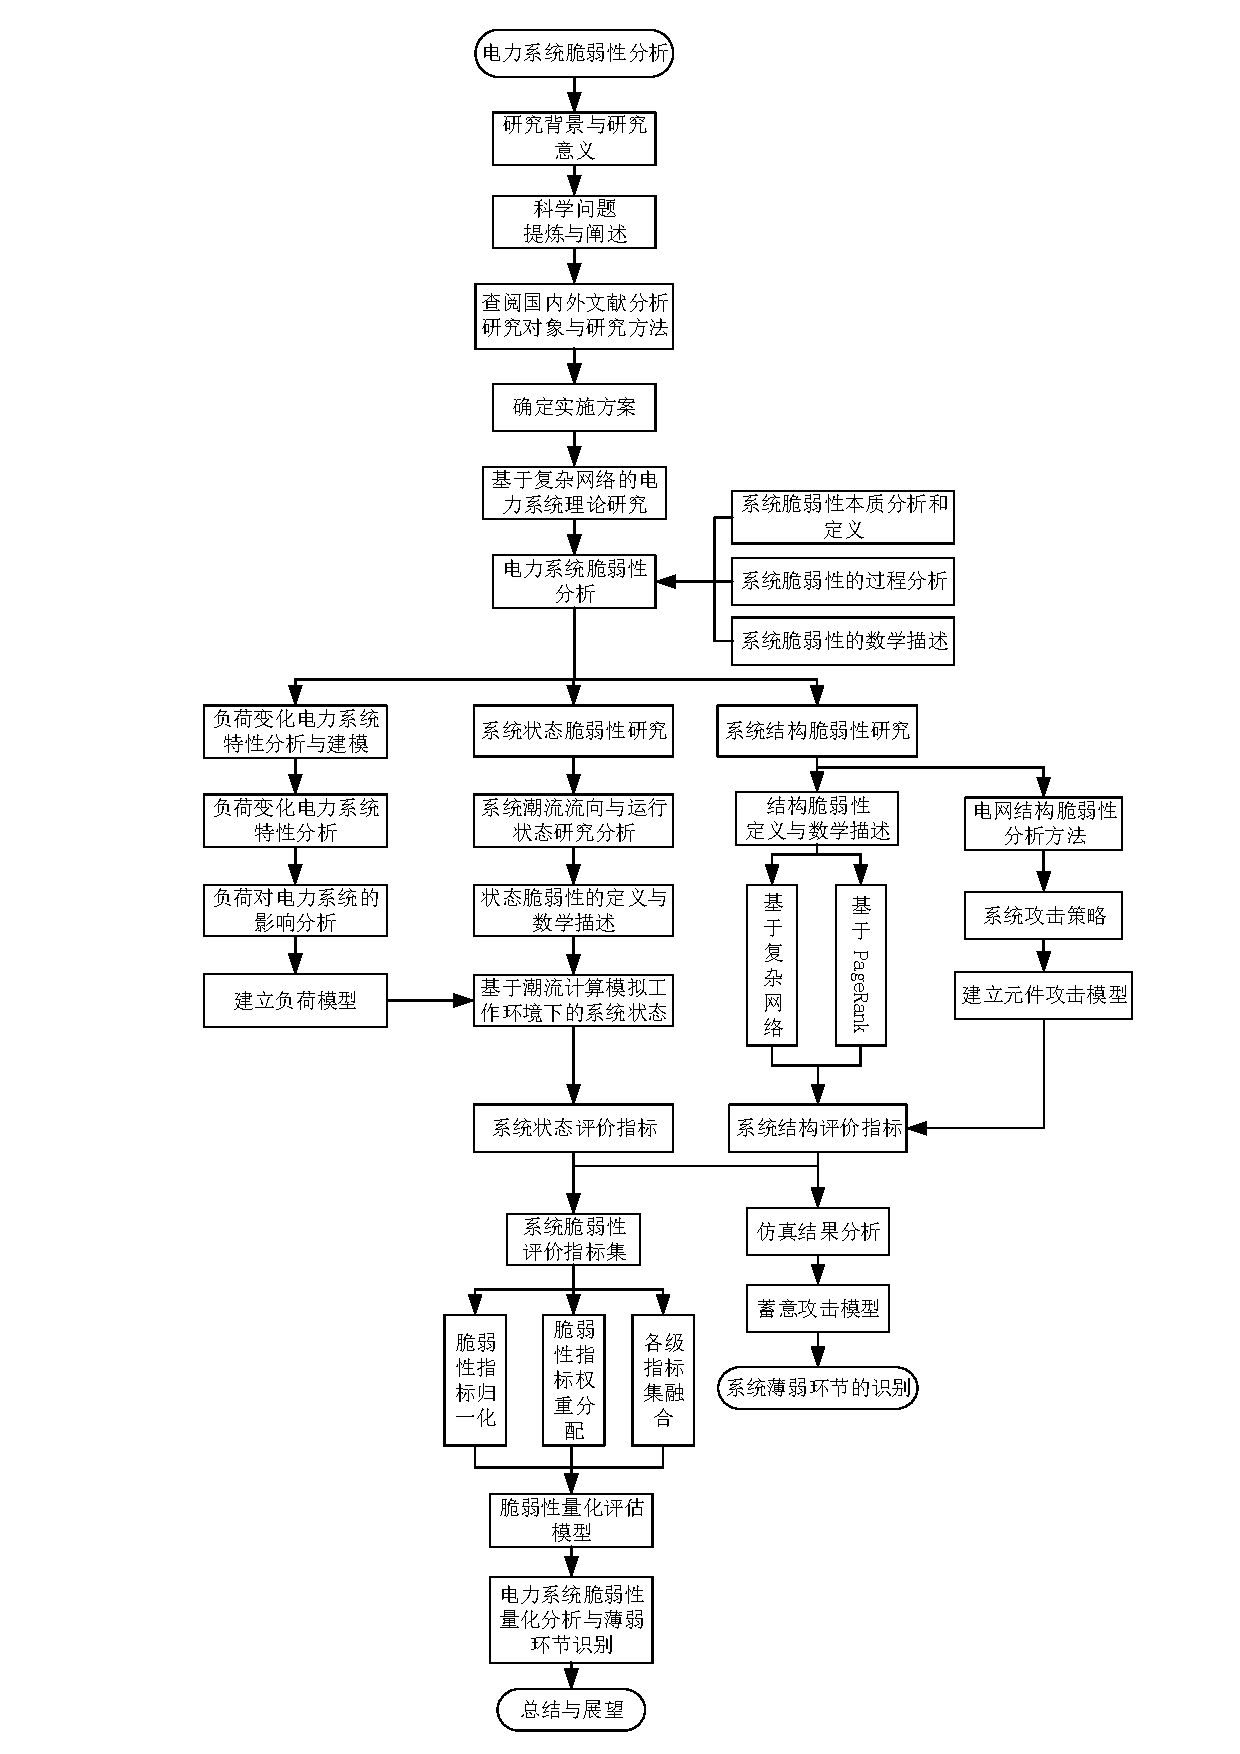
\includegraphics[height=23cm]{technicalRoute.pdf}
  \caption{技术路线图}
  \label{fig:technicalRoute}
\end{figure}

\chapter{基于复杂网络理论的电网模型验证分析}
\label{cha:model}

\section{引言}
\label{sec:index2}
经典的电力网络分析是基于基尔霍夫电流电压方程、固定的拓扑结构来进行分析的。其研究已形成了较为完善的体系\cite{refs60}。随着科学技术的不断发展,电力系统
变得越来越复杂、规模越来越大。在网络拓扑和分析计算上,经典的电力网络分析方法因节点和线路复杂度高的问题上已不再适用。而从复杂网络角度来看,电力系统可以
简化成一个由节点(母线)和边(支路)构成的网络。在复杂网络理论的基础上进行电网结构研究分析,已成为电网结构脆弱性分析的发展趋势。

电力系统作为典型的复杂网络,在研究电力系统脆弱性之初,有必要对复杂网络的相关概念进行阐述和分析。本章首先阐述复杂网络的基本概念,在此基础上分析其基本特征
参数。此外,基于复杂网络的建模方法,分析验证复杂网络的两类模型,小世界模型和无标度模型。最后,在基本特征参数的基础上,分析与描述复杂网络的脆弱性,并研究
其脆弱性常用指标,为后续章节的电力系统结构脆弱性分析实验打下基础。

\section{复杂网络基本概念}
\label{sec:powersys}
复杂网络理论是把一个复杂系统抽象为网络,将复杂系统内的各个元件视为网络的节点,将元件之间的联系抽象为复杂网络中连接各个节点的边,由此建立起复杂网络模型。
复杂网络的基本概念主要包括复杂网络的概念描述和统计描述,概念描述主要包括复杂网络语言描述和特点及特性描述。统计描述主要包括网络的基本特征参数和静
态特性,研究复杂网络的基本概念对分析后续电力系统脆弱性指标有着重要的意义。

\subsection{复杂网络概念描述}
\label{sec:composite}
复杂网络这一概念,人们试图严格去定义复杂系统,但直到现在还未充分认识和了解复杂网络,故难以给出其严格和实用的定义\cite{refs61}。目前普遍认同的是,钱学森
院士等人发起研究的系统科学研究领域——开放的复杂巨系统理论中对复杂网络的定义:具有自组织、自相似、吸引子、小世界、无标度中部分或全部性质的网络称为复杂网络
\footnote{摘自中文维基百科}。下面其性质进行具体阐述:

$(1)$自组织:对于这一概念,从不同学科角度来看会有不同的解读,我们从系统论的观点来看,“自组织”是指一个系统在内在机制的驱动下,自行从简单到复杂、从粗糙
向细致方向发展。不断提高自身的复杂度和精细度的过程。其与“他组织”的区别在于:“他组织”是靠外部指令而形成的组织,而“自组织”是系统按照内在机制自动形成的有序结构。
一个系统自组织属性愈强,其保持和产生新功能的能力也愈强。

$(2)$自相似:是指复杂网络的总体与部分、这一部分与另一部分之间的精细结构或性质所具有的相似性,或者可以这样理解:从整体中取出局部(局域)能够体现整体的基
本特征。

$(3)$吸引子:是微积分和系统科学论中的概念。一个系统有朝某个稳态发展的趋势,这个稳态叫做吸引子。吸引子是一个数学概念,描述系统运动的收敛类型,它存在于相平面。
简言之,吸引子是一个集合,当时间趋向于无穷大时,在任何一个有界集上出发的非定常流的所有轨迹都趋向于这个集合。

$(4)$小世界性:网络的小世界性是指对具有较短平均路径又具有较高聚类系数的网络性质的一种定义。平均路径长度和聚类系数会在下一小节展开描述。

$(5)$无标度性:网络的无标度性是指对网络的度分布符合幂律分布的复杂网络性质的一种定义。具体来讲,复杂网络只有少数节点拥有大量的连接,而大部分节点却很少。

% 在以上系统科学的角度理解的基础上,给出以下对复杂网络比较直观的特性论述:

%$(1)$开放性

%复杂系统是开放的,受外界影响,复杂系统及其子系统与系统的环境之间有物质、能量和信息的交换。

%$(2)$复杂性

%复杂系统中的子网络的种类繁多,子网络之间存在多种形式、多种层次的交互作用。

%$(3)$进化涌现性

%在特定条件下,系统中各元件或各子系统之间相互作用。在此期间会有微小变化,但系统能自组织、自加强、自协调,并随之扩大、发展,发生质变。这种质变,在复杂系统中称为
%涌现。


\subsection{复杂网络统计描述}
\label{sec:feature}
在刻画复杂网络结构的统计特性上提出了许多概念和特征参数,其中包含四个基本的特征参数:度及度分布、平均路径长度、聚类系数和介数及介数分布。一般一个无权无向的抽象网络用
$\boldsymbol{M}=(\boldsymbol{V}, \boldsymbol{E})$表示,$\boldsymbol{V}$为节点集合,$\boldsymbol{E}$为边集合。

$(1)$节点度及度分布:

节点$v_i$的度$k_i$定义为与该节点连接的所有节点的数量。直观来讲,一个节点的度越大,这个节点在某种情况下越重要。

网络的度分布可用分布函数$P(k)$来描述,$P(k)$的定义为网络中度为$k$的节点数量在整个网络中所占的比例,换言之,网络中节点度为$k$的概率为$P(k)$

$(2)$平均路径长度:

将网络中两个节点$v_i$和$v_j$之间的距离$d_{ij}$定义为连接这两个节点的最短路径上的边数,$L$定义为所有节点对之间最短距离的均值。

\begin{equation}
    \label{equ:chap3:feature}
    L=\frac{1}{C_N^2} \sum_{i \neq j} d_{i j}
\end{equation}

式中:$N$为网络节点数。

$(3)$聚类系数:

聚类系数是一个表征两个节点间连接紧密程度的特征参数。当节点$v_i$的节点度为$k_i$,那么相邻节点之间的边数最大为$\frac{k_i(k_i-1)}{2}$,假设节点$v_i$的$k_i$和邻居节点
之间实际存在的边数为$E_i$,那么节点$v_i$的聚类系数定义为:$C_i=\frac{2E_i}{k_i(k_i-1)}$。网络的聚类系数为:

\begin{equation} 
    \label{equ:chap3:feature}
    C=\frac{1}{N} \sum_{i=1}^N C_i
\end{equation}

式中:$N$为网络节点数。

$(4)$介数及介数分布

网络中的不相邻节点$v_i$和$v_j$之间的最短路径会途经某些节点或边,如果某些节点$v$或边$e$被其他许多最短路径经过,则表示该节点对网络的贡献较大,重要性也越高。将节点介数
$B(v)$和边介数$B(e)$分别定义为:

\begin{equation} 
    \label{equ:chap3:feature}
    B(v)=\sum_{i \neq j\in V} \frac{\sigma_{ij}(v)}{\sigma_{ij}} 
\end{equation}
\begin{equation} 
    \label{equ:chap3:feature}
    B(e)=\sum_{i \neq j\in V} \frac{\sigma_{ij}(e)}{\sigma_{ij}} 
\end{equation}

式中:$\sigma_ij$是节点$v_i$和$v_j$间最短路径的数量,$\sigma_ij(v)$是节点$v_i$和$v_j$通过节点v的最短路径数量,$\sigma_ij(e)$是节点$v_i$和$v_j$通过支路e的最短路
径数量。

\section{基于复杂网络理论的电网模型性质分析}
\label{sec:wind}

\subsection{小世界模型}
\label{sec:windEffects}
在复杂网络理论中,将现实中的复杂网络抽象成节点和边,比如人脉、互联网和电网。Watts和Strogatz将具有高聚集程度、小平均距离的这一类网络称为小世界网络\cite{refsWS}。提出小世界模型
(WS模型)。其构造过程为:首先构造一个最近邻连接的规则网络,然后以概率$p$随机断开网络上的一条边后重新连接边。当$p$为0时,网络为规则网络,当$p$为1时,网络为随机网络。当$0<p<1$
时,网络为小世界网络。当重连概率$p$介于0—1变化时,网络模型的聚类系数和平均距离也在发生变化,其演变过程如图\ref{fig:SW}所示。因小世界网络具有聚集系数高、平均距离小的特征,所以
小世界网络体现出少数随机连接的重要作用。
\begin{figure}[H] % use float package if you want it here
    \centering
    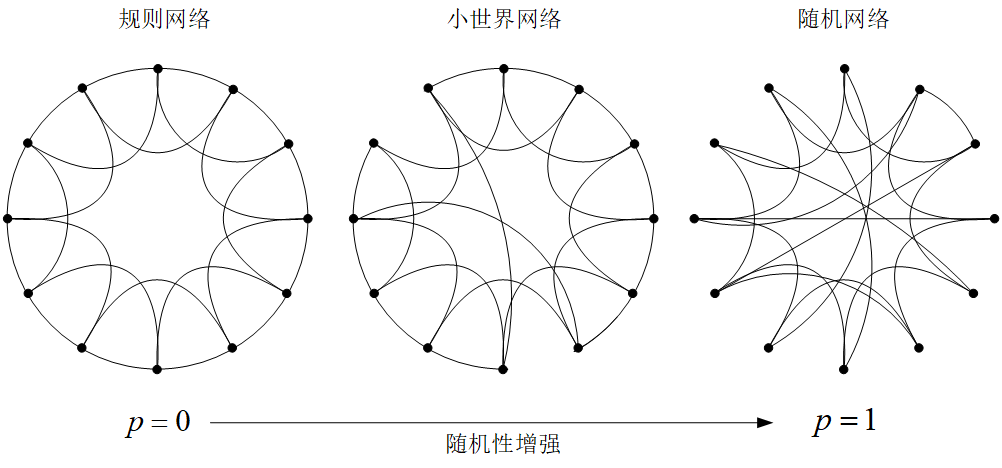
\includegraphics[width=14cm,height=6.5cm]{SW_network.png}
    \caption{小世界网络模型示意图}
    \label{fig:SW}
  \end{figure}

下面进行算例分析,取节点数$N = 1000$,初始网络规则的度$K = 6$,重连概率$p$从0-1依此增加,验证聚类系数$C$和平均距离$L$的变化过程。其验证结果如图\ref{fig:CL}所示。
\begin{figure}[H] % use float package if you want it here
    \centering
    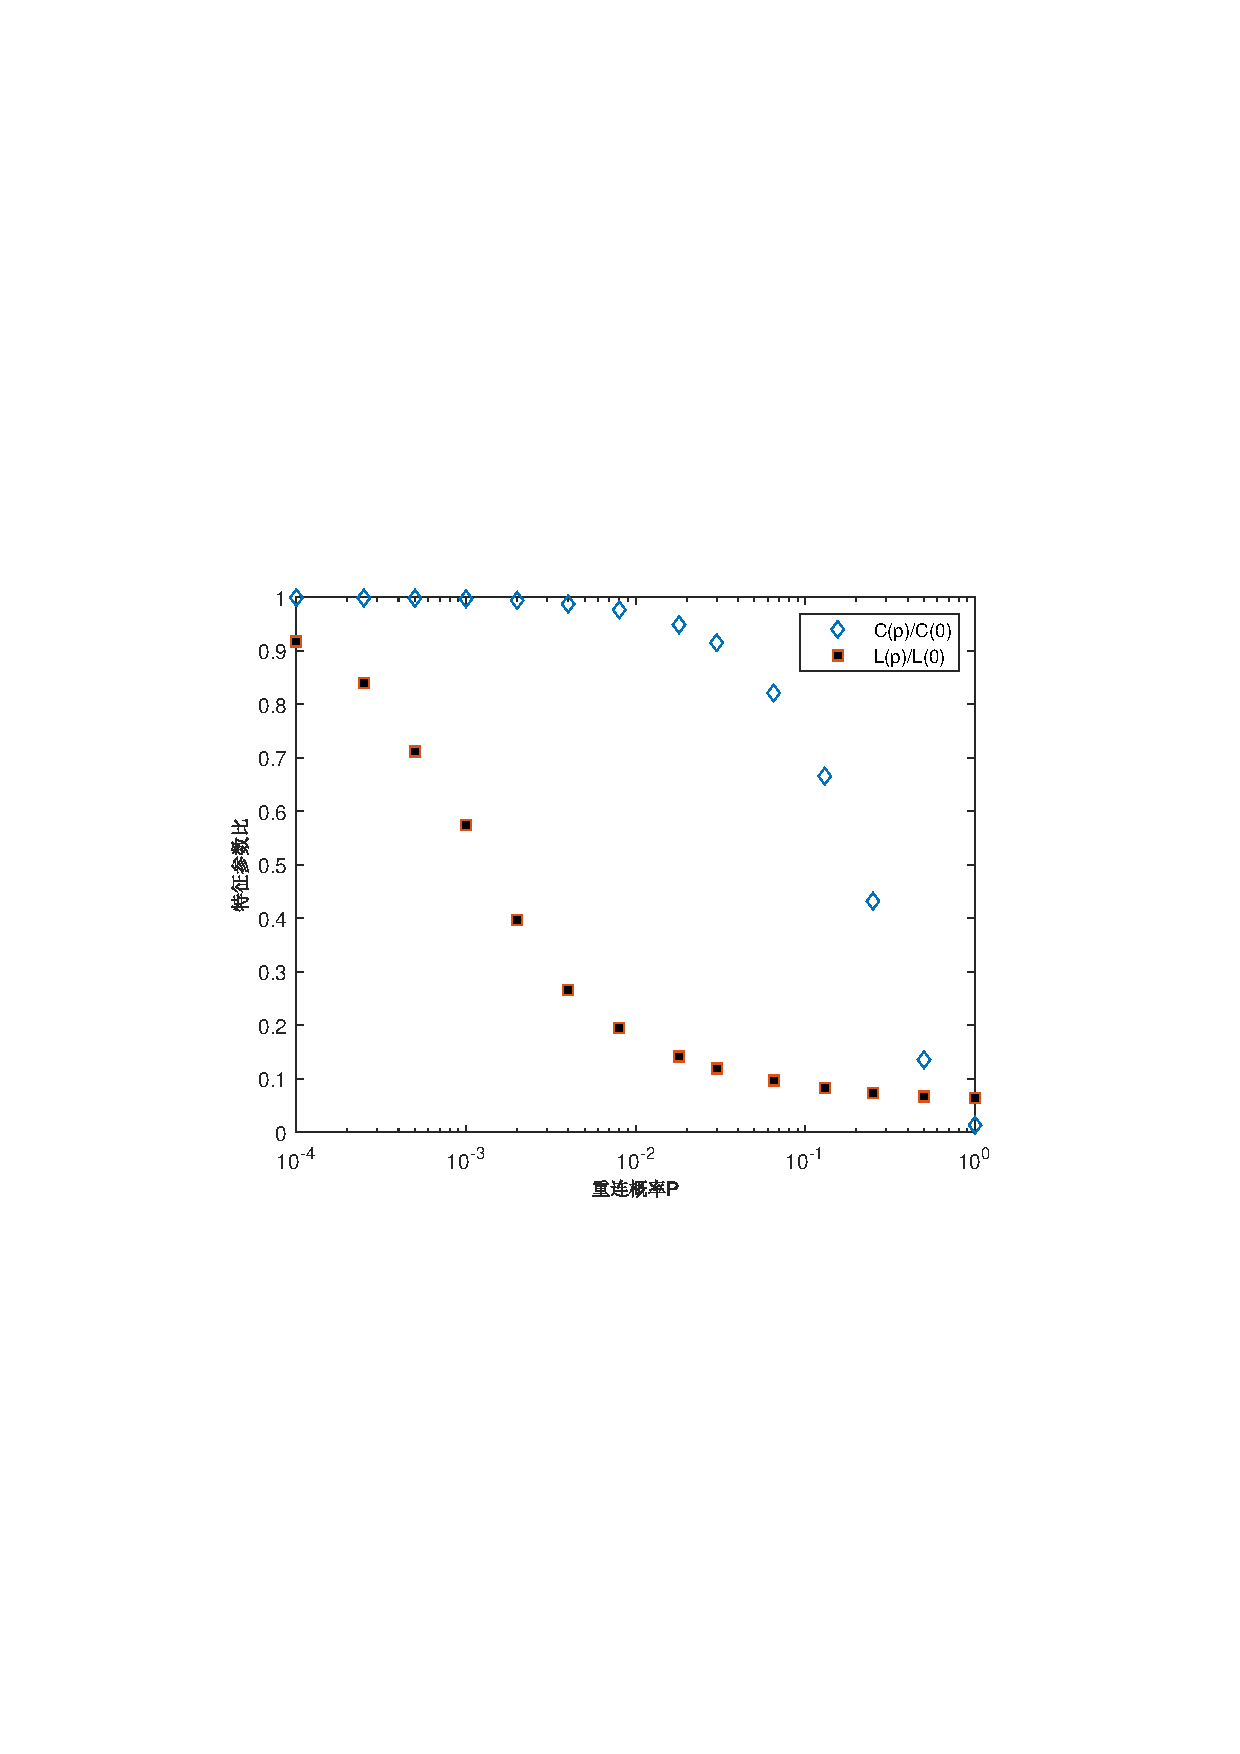
\includegraphics[]{CL.pdf}
    \caption{各重连概率$p$值下聚类系数$C$和平均路径长度$L$的变化趋势}
    \label{fig:CL}
\end{figure}

从图\ref{fig:CL}可以看出,随着重连概率$p$的增加,规则网络经历了从小世界网络到随机网络演变的过程,小世界网络相比于随机网络具有高聚集系数的特征,而相比于规则网络又具有
小平均距离的特征。其表达式如下:
\begin{equation}
\label{equ:chap2:CL}
 C\gg C_{random} \quad \quad\quad L \ll L_{regular}
\end{equation}

小世界网络模型在具体网络的应用方面具有很重要的现实意义。在网络动力学原理中,一般的网络当节点出现故障时,其影响范围很小。而在小世界网络中,由于节点间存在长程连接,节点故障
可能会快速传播到网络其他区域,进而引起网络的连锁故障。小世界网络的特征路径长度和聚类系数与故障传播的深度和广度由密切关系。一般地,特征路径路径长度越小,则故障传播就越深;
聚类系数越大,故障传播就越广\cite{refsWS1}。

为验证电力系统网络具有小世界特性,下面通过MATLAB工具分别利用$IEEE$30、$IEEE$39和$IEEE$57标准算例模型进行验证,并与相同节点数的规则网络和
随机网络进行对比分析。$IEEE$30、$IEEE$39和$IEEE$57标准算例模型的边数分别为41、46、81。规则网络采用的是最近邻耦合网络,所有的节点只与其最近的$K$个邻居节点相连,因此令规则网络
的边数约等于标准电网模型的边数,$K=2$。并在此规则网络上构建随机网络,重连概率$p$为$0$,取1000次仿真计算结果的平均值为最终值,其仿真结果如表\ref{tab:ieee}、\ref{tab:regular}、\ref{tab:random}所示。
\begin{table}[htb]
    \centering
    \caption{$IEEE$标准算例特征参数计算结果}
    \label{tab:ieee}
      \begin{tabular}{C{3cm}C{3cm}C{3cm}C{3cm}}
        \toprule
        $IEEE$标准算例      & $IEEE$30节点 & $IEEE$39节点 & $IEEE$57节点\\
        \midrule
        聚类系数($C$)       & 0.2348       & 0.0385      & 0.1222 \\
        平均路径长度($L$)   & 3.3057       & 4.7490      & 4.9536 \\
        \bottomrule
      \end{tabular}
  \end{table}

\begin{table}[htb]
    \centering
    \caption{规则网络特征参数计算结果}
    \label{tab:regular}
      \begin{tabular}{C{3cm}C{3cm}C{3cm}C{3cm}}
        \toprule
        规则网络            & 30节点        & 39节点      & 57节点\\
        \midrule
        聚类系数($C$)       & 0             & 0           & 0 \\
        平均路径长度($L$)   & 10.3333       & 13.3333      & 19.3333  \\
        \bottomrule
      \end{tabular}
\end{table}

\begin{table}[htb]
    \centering
    \caption{随机网络特征参数计算结果}
    \label{tab:random}
      \begin{tabular}{C{3cm}C{3cm}C{3cm}C{3cm}}
        \toprule
        随机网络            & 30节点        & 39节点      & 57节点\\
        \midrule
        聚类系数($C$)       & 0.0389       & 0.0275       &  0.0208 \\
        平均路径长度($L$)   & 7.6711        & 8.5568        & 9.1382  \\
        \bottomrule
      \end{tabular}
\end{table}

为了直观显示,规则网络、$IEEE$标准电网和随机网络聚类系数和平均路径长度的对比值如图\ref{fig:Cluster}、\ref{fig:L_mean}所示。
\begin{figure}[H] % use float package if you want it here
    \centering
    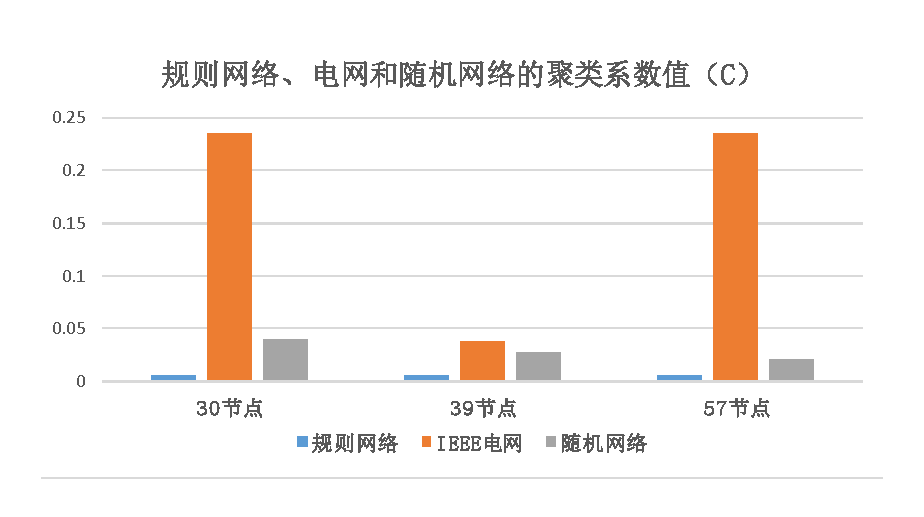
\includegraphics[width=10cm,height=5cm]{Cluster.pdf}
    \caption{规则网络、电网和随机网络的聚类系数结果图}
    \label{fig:Cluster}
\end{figure}

\begin{figure}[H] % use float package if you want it here
    \centering
    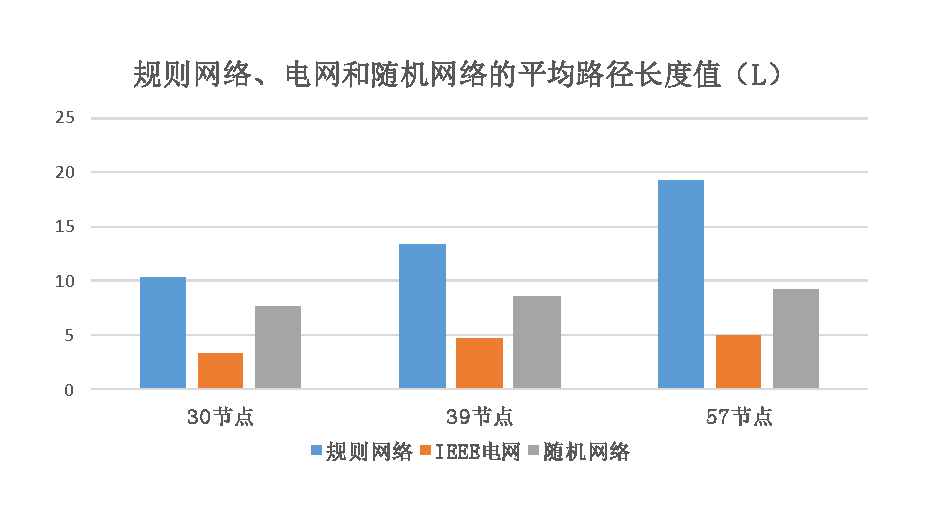
\includegraphics[width=10cm,height=5cm]{L_mean.pdf}
    \caption{规则网络、电网和随机网络的平均路径长度结果图}
    \label{fig:L_mean}
\end{figure}

从表\ref{tab:regular}可以看出,在规则网络中,节点30、39、57网络的聚类系数均为0,这是由于每个节点的度数都为 2,因此该规则网络中任意节点的邻居节点都互相不连接,故聚类系数为0。
从图\ref{fig:Cluster}和图\ref{fig:L_mean}验证了式\ref{equ:chap2:CL}的正确性,可以直观看出,实际电网系统的聚类系数远大于随机网络的聚类系数,其平均路径长度远小于规则网络的路径长度,
换句话说,电力系统网络相比于随机网络具有高聚集系数的特征,而相比于规则网络又具有小平均距离的特征,因此,验证得到电网模型为小世界网络,具有小世界性。较小的平均距离和较大的聚类系数,在
电网局部发生故障时,其故障具有较大的传播范围和传播速度。这对于研究电网的结构脆弱性具有重要的应用意义。

\subsection{无标度模型}
\label{sec:windModel}
在规则网络中,各节点的度数相同,因此规则网络的度分布集中在一个固定值上。随机网络中,由于其网络的边是以相同概率进行重连的,所以随机网络的度分布大致集中在一个概率范围内。在复杂网络理论中,
大多数现实中的网络的度数呈幂律分布,如式\ref{equ:chap2:milv}所示。因为这些网络的节点没有明显的标度,所以这种网络被称为无标度网络。
\begin{equation}
\label{equ:chap2:milv}
P(k) \propto k^{-r}
\end{equation}

在复杂网络理论中,对无标度的鲁棒性进行分析发现,随机攻击对于无标度网络结构的连通性影响很小,而攻击指定的关键环节将会对网络连通性影响很大。在电网中,电网关键节点结构的变化会对网络的连通性
造成极大的影响,进而影响电网的运行状态导致负荷损失。因此,无标度网络中的关键环节可视为电网模型的脆弱环节。下面将对电网模型的无标度性进行验证。

为了研究电网结构脆弱性,将验证电网模型的无标度特性,为此,本文选取$IEEE13659pegase$节点标准算例进行实验,通过$MATLAB$计算电网模型中各节点的度,进而得到电网的度分布结构,实验结果如图
\ref{fig:dufenbu}所示。
\begin{figure}[H] % use float package if you want it here
  \centering
  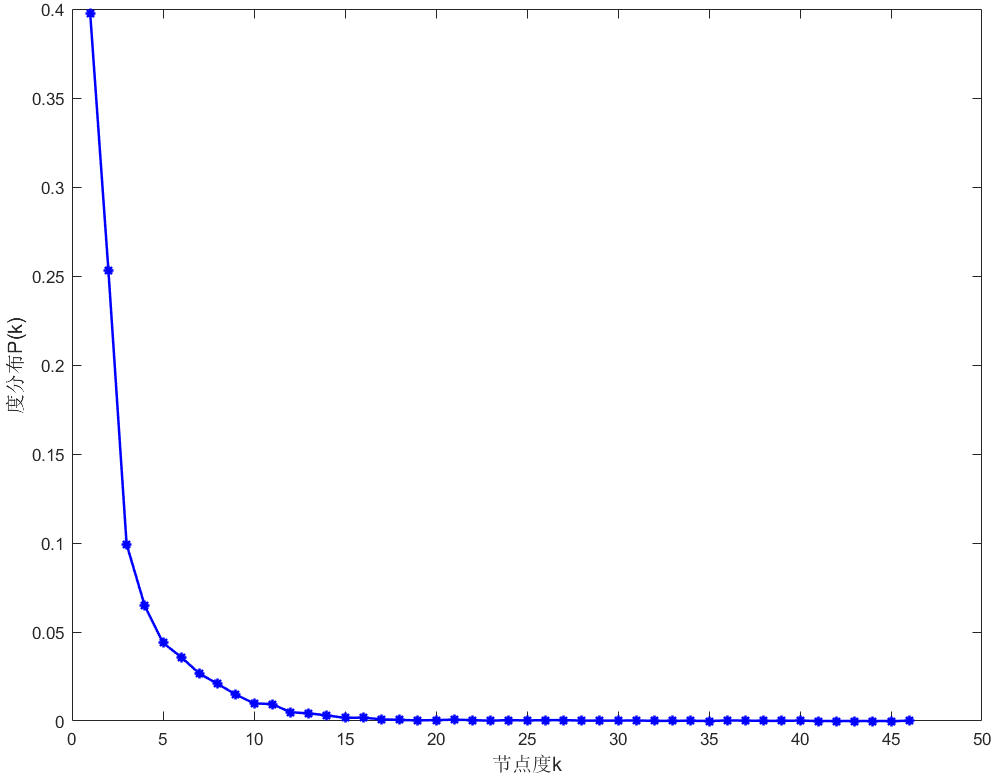
\includegraphics[width=12cm,height=8cm]{dufenbu.png}
  \caption{$IEEE13659pegase$标准算例节点度分布图}
  \label{fig:dufenbu}
\end{figure}

从图\ref{fig:dufenbu}可以看出,将近$40\%$节点度为1,节点度为2的占到了$25\%$以上,节点度为3的约占$10\%$,剩下的约占$25\%$,下面对$IEEE13659pegase$标准算例节点度分布进行幂函数拟合。
其拟合结果如图所示。
\begin{figure}[H] % use float package if you want it here
  \centering
  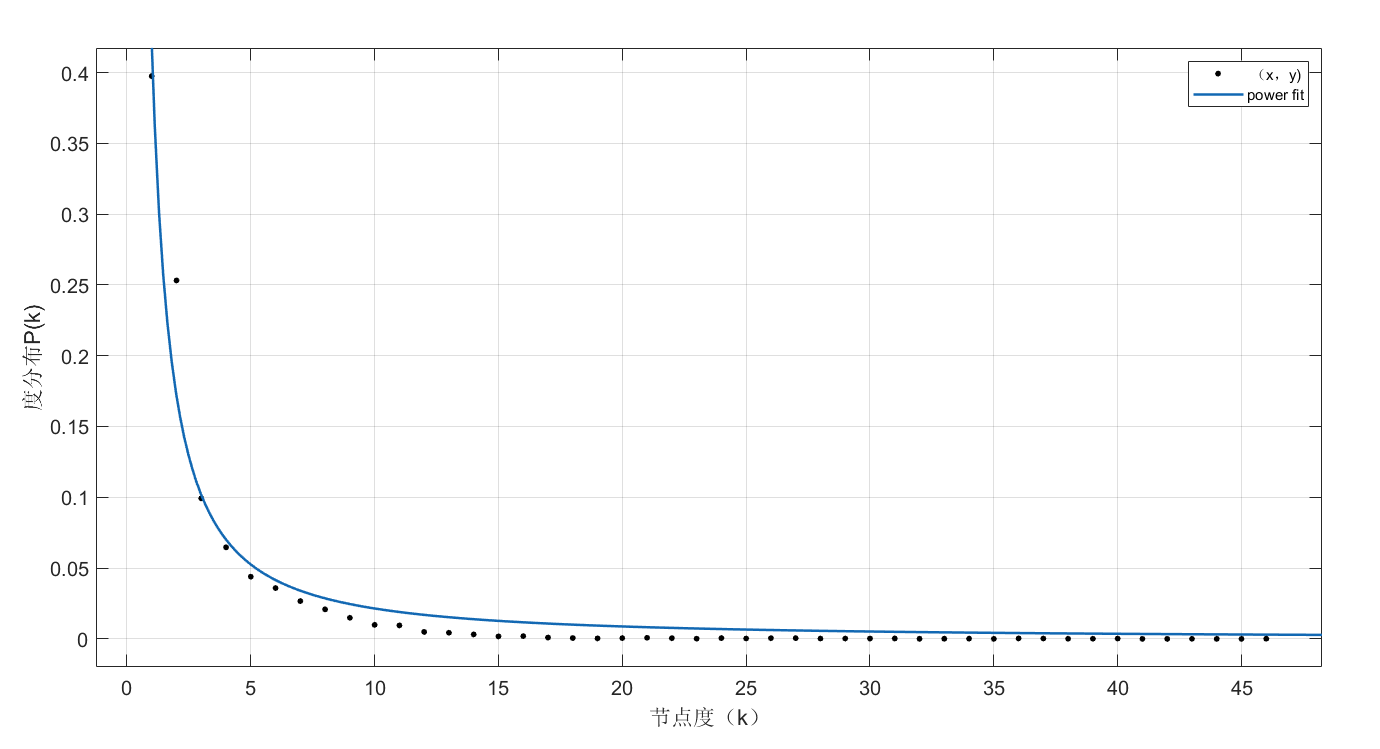
\includegraphics[width=14.7cm,height=8cm]{power_fit.png}
  \caption{$IEEE13659pegase$标准算例节点度分布拟合图}
  \label{fig:fower_fit}
\end{figure}

利用IEEE13659pegase标准算例,得到其度分布示意图,其趋势变化服从幂律分布,对数据进行数据拟合得到$p(k)=a k^{b}(a=0.4206, b=-1.292)$ 置信度为$95\%$,服从幂律分布。

在复杂网络理论中,无标度特性反映出电网具有严重的异质性,其各节点之间的连接状况(度数)具有严重的不均匀分布性:网络中少数称之为Hub点的节点拥有极其多的连接,而大多数节点只有很少量的连接。
少数Hub点对无标度网络的运行起着主导的作用。从广义上说,无标度网络的无标度性是描述大量复杂系统整体上严重不均匀分布的一种内在性质。这也表明了电网作为无标度网络的一种,当其面临蓄意的节点
攻击时较为脆弱,面临随机攻击时鲁棒的特点。通过验证电网的无标度特性,对本文提出脆弱性指标和研究电网结构脆弱性具有重要意义。

\section{复杂网络的脆弱性描述}
\label{sec:load}



\subsection{脆弱性概念}
\label{sec:loadEffect}




\subsection{脆弱性常用指标}
\label{sec:loadModel}




\section{本章小结}
\label{sec:sum2}







%%% 其它部分
\backmatter

% 致谢
\begin{acknowledgement}
在此论文成稿之际,谨向我尊敬的导师苏永清副教授致以最诚挚的感谢!本文的选题内容、研究思路与分析过程均在苏老师的悉心指导下完成。
在两年的课题研究过程中,始终得到苏老师科研上的帮助与指导。苏老师渊博的学识、严谨的治学理念以及以身作则的工作态度,深深地感染
了我,在此我谨向您致以深切的感谢与诚挚的敬意。感谢岳继光教授与董延超副教授在工程项目及日常生活中给予我的帮助。你们严谨的学术
态度与踏实的工作作风为实验室建立了严谨求实的研究氛围,感谢你们为实验室的辛勤付出。

感谢同门师兄张鲲鹏与陈峰在研究课题中的指导,感谢刘志刚与徐晨剑师兄在工程项目中对我的帮助,徐晨剑师兄的论文~\LaTeX~模板使我受
益匪浅。感谢侯培鑫博士在学术方法上对我的提点以及多次赠书之情,感谢王森博博士与王栗博士在项目中的指导与帮助,祝你们顺利毕业。
感谢同届研究生施梁、汪嬴、唐丹旭、吴琛浩,同窗之情,友谊长存,祝你们今后工作顺利。感谢刘雪娇与穆慧华两位师妹在~502~研究所与
~811~研究所工程项目中的协助。感谢同济大学先进测控技术课题组徐刚、陈策、乔琪、张爽、武新然、李炅聪等全体成员,伴我度过了难忘的
研究生时光,在此祝大家前程似锦,幸福快乐。

同时感谢张志明老师对我在虚拟仪器俱乐部工作的支持与帮助,感谢黄蓉荣师姐、吉方成师兄与陈阳师兄在虚拟仪器俱乐部对我的指导与帮助,
祝同济大学虚拟仪器俱乐部越办越好。感谢贾青老师与同济大学~PACE~中心对我工作上的支持,感谢张世博师兄在~Urban Flexible Vehicle~项目
中的帮助,那些熬夜调车的夜晚至今历历在目。

此外,感谢好友狄宗林与邵瑶夏,与你们相识让我看到青年才俊们的努力与拼搏,祝你们最终实现梦想。感谢好友~Paolo Curti~在意大利的
热情招待,Omegna~湖畔的烟花绚烂依旧。


最后,要感谢我的父亲母亲,是你们的支持才使我能走到今天。养育之恩,无以为报,你们健康快乐是我最大的心愿。在未来的学习、
工作与生活中,我会继续锐意进取,成于精勤、止于至善。


~~\\


\rightline{赵闻达\qquad \quad}

\rightline{2018年3月于上海嘉定}
\end{acknowledgement}

% 参考文献
\printTJbibliography


% 附录
\begin{appendix}
\chapter{$IEEE39$系统数据}
\label{cha:engorg0}

\section{$IEEE$39系统节点}
\label{sec:lp0}

\begin{table}[H]
  \centering
  \caption{$IEEE$39系统发电节点}
  \label{tab:chap5:generator39}
    \begin{tabular}{C{3cm}C{3cm}C{3cm}}
\toprule
\textbf{节点名}        &\textbf{额定有功功率($MW$)}      &\textbf{是否为平衡节点}         \\
\midrule
            30        &250 &否\\
            31        &677.81 &是 \\
            32        &650  &否 \\
            33        &632  &否 \\
            34        &508   &否\\
            35        &650 &否\\
            36        &560 &否\\
            37        &540 &否\\
            38        &830 &否\\
            39        &1000 &否\\
\bottomrule
\end{tabular}
\end{table}

\begin{table}[H]
  \centering
  \caption{$IEEE$39系统负荷节点}
  \label{tab:chap5:load39}
    \begin{tabular}{C{1.2cm}C{2.4cm}C{2.4cm}C{1.2cm}C{2.4cm}C{2.4cm}}
\toprule
            \textbf{节点名}        &\textbf{额定有功功率($MW$)}      &\textbf{额定无功功率($MVar$)}   & \textbf{节点名}        &\textbf{额定有功功率($MW$)}      &\textbf{额定无功功率($MVar$)}       \\
\midrule
            1        &97.6 &44.2 & 16        &329.0 &32.3\\
            2        &0.0 &0.0 &17        &0.0 &0.0\\
            3        &322.0  &2.4 &18        &158.0 &30.0\\
            4        &500.0  &184.0 &19        &0.0 &0.0\\
            5        &0.0 &0.0 &20        &680.0 &103.0\\
            6       &0.0 &0.0 &21        &274.0 &115.0\\
            7        &233.8 &84.0 &22        &0.0 &0.0\\
            8        &522.0 &176.6 &23        &247.5 &84.6\\
            9        &6.5 &-66.6 &24        &308.6 &-92.2\\
            10        &0.0 &0.0 &25        &224 &47.2\\
            11        &0.0 &0.0 &26        &139 &17\\
            12        &8.53 &88.0 &27        &281 &75.5\\
            13        &0.0 &0.0 &28        &206 &27.6\\
            14        &0.0 &0.0 &29        &283.5 &26.9\\
            15        &320.0 &153.0 & & &\\
\bottomrule
\end{tabular}
\end{table}

\chapter{$IEEE118$系统数据}
\label{cha:engorg}

\section{$IEEE$118系统发电节点}
\label{sec:lp}

\begin{table}[H]
\centering
\caption{$IEEE$118系统发电节点}
\label{tab:chap5:generator118}
\begin{tabular}{C{1.4cm}C{2.4cm}C{2.2cm}C{1.4cm}C{2.4cm}C{2.2cm}}
\toprule
\textbf{节点名} & \textbf{额定有功功率(MW)} & \textbf{ 是否是平衡节点 } & \textbf{节点名} & \textbf{额定有功功率(MW)}  & \textbf{ 是否是平衡节点 } \\
\midrule
1   & 0          & 否       & 65  & 391        & 否       \\
4   & 0          & 否       & 66  & 392        & 否       \\
6   & 0          & 否       & 69  & 516.4      & 是       \\
8   & 0          & 否       & 70  & 0          & 否       \\
10  & 450        & 否       & 72  & 0          & 否       \\
12  & 85         & 否       & 73  & 0          & 否       \\
15  & 0          & 否       & 74  & 0          & 否       \\
18  & 0          & 否       & 76  & 0          & 否       \\
19  & 0          & 否       & 77  & 0          & 否       \\
24  & 0          & 否       & 80  & 477        & 否       \\
25  & 220        & 否       & 85  & 0          & 否       \\
26  & 314        & 否       & 87  & 4          & 否       \\
27  & 0          & 否       & 89  & 607        & 否       \\
31  & 7          & 否       & 90  & 0          & 否       \\
32  & 0          & 否       & 91  & 0          & 否       \\
34  & 0          & 否       & 92  & 0          & 否       \\
36  & 0          & 否       & 99  & 0          & 否       \\
40  & 0          & 否       & 100 & 252        & 否       \\
42  & 0          & 否       & 103 & 40         & 否       \\
46  & 19         & 否       & 104 & 0          & 否       \\
49  & 204        & 否       & 105 & 0          & 否       \\
54  & 48         & 否       & 107 & 0          & 否       \\
55  & 0          & 否       & 110 & 0          & 否       \\
56  & 0          & 否       & 111 & 36         & 否       \\
59  & 155        & 否       & 112 & 0          & 否       \\
61  & 160        & 否       & 113 & 0          & 否       \\
62  & 0          & 否       & 116 & 0          & 否     \\
\bottomrule
\end{tabular}
\end{table}

\section{$IEEE$118系统负荷节点}
\begin{table}[H]
   \centering
   \caption{$IEEE$118系统负荷节点}
   \label{tab:chap5:load118}
     \begin{tabular}{C{1.2cm}C{2.4cm}C{2.4cm}C{1.2cm}C{2.4cm}C{2.4cm}}
\toprule
 \textbf{节点名}        &\textbf{额定有功功率($MW$)}      &\textbf{额定无功功率($MVar$)}   & \textbf{节点名}        &\textbf{额定有功功率($MW$)}      &\textbf{额定无功功率($MVar$)}       \\
\midrule
2  & 20 & 9  & 57  & 12 & 3  \\
3  & 39 & 10 & 58  & 12 & 3  \\
5  & 0  & 0  & 60  & 78 & 3  \\
7  & 19 & 2  & 63  & 0  & 0  \\
9  & 0  & 0  & 64  & 0  & 0  \\
11 & 70 & 23 & 67  & 28 & 7  \\
13 & 34 & 16 & 68  & 0  & 0  \\
14 & 14 & 1  & 71  & 0  & 0  \\
16 & 25 & 10 & 75  & 47 & 11 \\
17 & 11 & 3  & 78  & 71 & 26 \\
20 & 18 & 3  & 79  & 39 & 32 \\
21 & 14 & 8  & 81  & 0  & 0  \\
22 & 10 & 5  & 82  & 54 & 27 \\
23 & 7  & 3  & 83  & 20 & 10 \\
28 & 17 & 7  & 84  & 11 & 7  \\
29 & 24 & 4  & 86  & 21 & 10 \\
30 & 0  & 0  & 88  & 48 & 10 \\
33 & 23 & 9  & 93  & 12 & 7  \\
35 & 33 & 9  & 94  & 30 & 16 \\
37 & 0  & 0  & 95  & 42 & 31 \\
38 & 0  & 0  & 96  & 38 & 15 \\
39 & 27 & 11 & 97  & 15 & 9  \\
41 & 37 & 10 & 98  & 34 & 8  \\
43 & 18 & 7  & 101 & 22 & 15 \\
44 & 16 & 8  & 102 & 5  & 3  \\
45 & 53 & 22 & 106 & 43 & 16 \\
47 & 34 & 0  & 108 & 2  & 1  \\
48 & 20 & 11 & 109 & 8  & 3  \\
50 & 17 & 4  & 114 & 8  & 3  \\
51 & 17 & 8  & 115 & 22 & 7  \\
52 & 18 & 5  & 117 & 20 & 8  \\
53 & 23 & 11 & 118 & 33 & 15 \\
\bottomrule
\end{tabular}
\end{table}

\end{appendix}

% 个人简历
\begin{resume}
\resumeitem{个人简历:}
\noindent 1995 年 3 月 1 日出生于山东省临沂市。\\
\noindent 2017 年 6 月本科毕业于山东科技大学获得学士学位。\\
\noindent 2017 年 9 月进入同济大学攻读硕士学位至今。


\resumeitem{参与项目:} % 有就写,没有就删除
\begin{enumerate}[{[}1{]}]
\item 国家重点研发计划“产品全生命周期模型管理技术与系统”项目
\item 航天基金“航天卫星电源系统性能分析”项目
\end{enumerate}

\end{resume}

\end{document}
